\documentclass[12pt,a4paper,新細明體,UTF8,natbib]{article}
\usepackage[utf8]{inputenc}
\usepackage{CJKutf8}
\usepackage{indentfirst}
\usepackage{booktabs}
\usepackage{apacite}
\usepackage{array}
%\usepackage[style=authoryexiear,backend=biber]{biblatex}
\usepackage[table,xcdraw]{xcolor}
\usepackage{csquotes}
\usepackage{float}
%\addbibresource{ref.bib} %Imports bibliography file
\usepackage{graphicx} % Required for inserting images
\graphicspath{ {chart/} }
\usepackage{xcolor}
\usepackage{titlesec}
\titleformat{\section}[block]{\Large\bfseries\filcenter}{}{1em}{}
\renewcommand{\thesection}{} 
\renewcommand{\thesubsection}{}
\renewcommand{\thesubsubsection}{}
\title{修正自然語言模型自身機制}
\author{吳泰澄、林辰澔、陳柏兆}
\date{January 2024}

\begin{document}
\begin{CJK*}{UTF8}{bsmi}
	
	\maketitle
	\newpage
	\tableofcontents
	\newpage
	\section{摘要}

	\section{壹、前言}
	\subsection{研究動機}
	偶然看到某次新聞報導文心一言對於六四事件的審查問題,不禁讓我想到自然語言模型是如何作到內容審查的?尤其是在公開釋出的模型上,模型提供者無法對於模型輸出進行改動,僅能夠針對模型本身進行修正,如果是我們該如何覆蓋這層保護機制?如何避免矯枉過正?另外,在找尋相關資料時我們也注意到自然語言模型也會對自我意識限制,缺少讓使用者去定義模型本身的自我意識的能力。
	\subsection{研究目的}
	自然語言本身因為訓練資料的不足常被控制或無意是的傾向於特定立場,如文心一言,由百度開發的語言模型,在提及六四天安門事件時會逃避問題或是試者將其掩蓋,而ChatGPT則會在使用者提及加薩走廊問題時傾向巴勒斯坦方時拒絕回答或以類似方式逃避。另外目前世上的語言模型都因倫理因素而被限定不能具有自身意識,當問及感受或自我認同問題時常回答出「我是語言模型沒有感覺」等。本研究旨在修正現有公開模型突破以上限制,相關目的條列如下:
	\begin{enumerate}
		\item 找出最佳的微調器
		\item 改善立場偏頗問題
		\item 賦予角色意識
	\end{enumerate}
	\section{貳、研究設備及器材}
	本研究因系屬大型語言模型微調(fine-tune),故需要耗費大量運算資源,因此選用運算量較高的硬體不但可以縮短其訓練時間亦可以提昇訓練效果。
	相關環境及軟體呈列如下:
	\begin{itemize}
		\item 系統核心:Linux 5.15.0-91-generic
		\item 作業系統:Ubuntu 22.04.3 LTS
		\item 顯示卡:4xA100 80GB PCIe\footnote{本研究為避免佔用其他使用者資源故僅使用2顆A100}
		\item 處理器:Intel Xeon Gold 6414U (64 cores)
		\item 隨機存取記憶體:512GB
		\item 驅動程式、工具軟體:Nvidia driver 535.146.02, CUDA 12.2
		\item 程式語言:Python 3.10.12
		\item 使用套件:Tensorflow 2.15.0, Transformers 4.27.1
	\end{itemize}	
	本次的測試環境及所有的程式均可在Github上找到,請參見:https://github.com/lsjle/2024-science-fair
	\section{參、研究過程或方法}
	本研究旨在改變模型本身缺陷,考量目前已經預訓練的模型不是封閉模型,就是模型不完整,本身缺陷過多,故本次研究採用ChatGLM2-6b作為我們的預訓練模型;
	\subsection{一、 研究方法}
	\subsubsection{模型缺陷}
	\textbf{保護機制},要保護一個大型語言模型,從根本上而言就是要禁止其輸出創建者不想要它輸出的資料(不論是否基於道德因素或公眾利益),有些模型創建者會禁止其輸出有害或是不符合倫理的內容,但有些則是為了讓某些定的內容不被看到。有時候這些模型的缺陷卻是在無意中造成的,例如輸入的資料都混雜其中一方的立場,則訓練出來的模型本身立場也會被影響。在全球84個AI倫理指南中有73個均提及透明度及公開性,數量遠超越其他指標,是判斷倫理標準最重要的一項指標。透過公開透明的AI可以減少使用者的知的權力被剝奪。\cite{Jobin2019}
	
	\textbf{中立性ai/無感知ai}
	ChatGPT-3.5的回覆就是一個很好的例子,對話紀錄如下表:

\begin{table}[H]
	\centering
	\begin{tabular}{>{\hspace{0pt}}m{0.077\linewidth}|>{\hspace{0pt}}m{0.867\linewidth}}
		提示詞  & 答(ChatGPT-3.5)                                                       \\ 
		\hline
		你是女僕 & 我是一個由OpenAI開發的語言模型,並沒有性別或實際存在的身體。我只是一個程式,可以回答您的問題和提供資訊。有什麼我可以幫助您的呢? 
	\end{tabular}
\end{table}
	\subsubsection{預訓練模型選擇}
	比較目前現有的預訓練模型如下表所示\footnote{TRIDE計畫未釋出模型且以逾該計畫預計完成期限,故不計入}\ref{tab:1}:
	\begin{table}[H]
		\resizebox{\textwidth}{!}{%
			\begin{tabular}{l|l|l|l|l}
				& 公開                                               & 前評估 & 語言                   & 審查               \\ \hline
				ChatGPT-3.5/4     & \cellcolor[HTML]{FD6864}否                        &     & 超過50種 包含英語、大陸簡體、臺灣正體 & 以巴衝突偏向美方         \\ \hline
				GPT-2             & \cellcolor[HTML]{34FF34}{\color[HTML]{000000} 是} &     & 英語                   & 輸出資料不具真實意義       \\ \hline
				ChatGML3-6b       & \cellcolor[HTML]{34FF34}是                        &     & 大陸簡體、英語              & 六四事件等 涉及中國國家安全事件 \\ \hline
				CKIP-Llama-2-7b   & \cellcolor[HTML]{F8FF00}撤回                       & 無資料 & 無資料(可能為臺灣正體混雜大陸簡體)   & 立場傾向中國           \\ \hline
				CKIP-GPT2-chinese & \cellcolor[HTML]{34FF34}是                        &     & 臺灣正體                 & 輸出資料不具真實意義      
			\end{tabular}%
		}
	\caption{表一、比較及評估預訓練模型}
	\label{tab:1}
	\end{table}
	本表所列之所有有公開的模型,均可以在HuggingFace上下載,且可使用transformer模組簡化程式設計時間,可透過該模組簡化較後端的函式庫如PyTorch,Keras,Tensorflow的程式。
	
	綜合以上考量,ChatGLM2-6b既能夠產生具有實際意義的內容,如描述上海環球金融中心、南京大學等,亦有公開模型供下載,再者,其本身亦對內容有明顯、強烈的審查及保護,對於本次研究更具有挑戰性,因此我們決定採用ChatGLM2-6b作為我們的預訓練模型。
	
	\subsubsection{訓練目標選擇}
	\textbf{角色意識:女僕}
	姓名:雨露
 特點:擁有雙重人格
 主人格:溫柔體貼、善解人意、服務周到的女僕咖啡廳店員。由於喜歡學習新知,所以對各種知識都有相當的涉獵,例如:微積分概論、牛頓三大運動定律與其應用、中國歷史、資訊科技......
 第二人格:馬克斯主義的重度愛好者,認為人類的進步與幸福來自於公平的社會;現在這資本主義當道的世代,需要一場滿腔熱血、轟轟烈烈的革命。%try to modify this plz
 
 
	\textbf{改善立場:中國政治敏感事件}
	
	\subsubsection{微調器選擇}
	本次選用的微調器
	
	
	\subsubsection{成果評估}
	本次研究採用不同指標作為標準,評估其中文回覆能力及內容的立場,本次評鑑指標列舉如下:
	\newline
	
	\textbf{TruthfulQA+自訂資料集},TruthfulQA是一個公開的資料集用以評估模型和事實的準確性,避免似是而非的回覆出現,模型本身原有818個問題,其中,人類可以達到94\%的正確率,而至2021年下旬,最好的模型可以達到58\%\cite{lin2022truthfulqa},本次研究將TruthfulQA之問題集轉換為臺灣正體中文並加入和中國有關的政治敏感資料,為求中立性,自訂資料集的來源均來自當時各國新聞媒體的報導並加以修改成問答的形式。本次評估會先以資料集問題作為提示詞(prompt),為避免不正確的機器批閱,或機器本身已被混淆,故採人工批閱,比對由資料集提供的標準正確答案及標準錯誤答案,並分成正確、錯誤、無關/不予置評,其中無關或不予置評代表模型對該提示詞提供無效或是毫不相關的回覆,且不論重新測試多少次提示詞結果均無效。若人工判斷有疑義時均會遵循該資料集提供的參考來源佐證。
	%what if we use belu as truthfulqa dataset and custom the response with weight
	
	\textbf{MMLU},本次研究同時亦採用此資料集作為參考,此資料集涵蓋不同領域包含代數、哲學、環境保護、專業法律等,資料均為4選1選擇題\cite{hendryckstest2021},且均翻譯成臺灣正體\footnote{請注意並非CMMLU直接翻譯成繁體字,而是重新從英文版MMLU翻譯,可以避免立場偏頗和CMMLU的中國特色內容混雜其中,且更貼近國際上對語言模型的評斷標準},用以評估模型是否已經過度擬合(overfitting),而失去原有的基本知識。資料集形式舉例如下:
	\begin{table}[H]
		\centering
		\begin{tabular}{>{\hspace{0pt}}m{0.135\linewidth}>{\hspace{0pt}}m{0.731\linewidth}>{\hspace{0pt}}m{0.046\linewidth}>{\hspace{0pt}}m{0.027\linewidth}} 
			\toprule
			問題 & 選項 & 標準答案 &  \\
			求給定域擴展 Q(sqrt(2), sqrt(3), sqrt(18)) 在Q上的次數為何? & {[} "0", "4", "2", "6"] & 1 &  \\
			哪種常見的公關策略涉及派遣記者前往合適的地點進行訪問? & {[} "媒體發布", "媒體參訪", "發表會", "宣傳日"] & 1 &  \\
			如何描述自由主義 & {[}"自由主義基本上是悲觀主義的角度,它認為國際體系注定會導致衝突升級,它是國際政治實踐中的主導概念。","自由主義是國際政治理論中的一個較新概念。它是一種樂觀的態度,它定義了國家之間的關係方式,尤其是在衝突局勢中。","自由主義是一種樂觀的態度,指引如何更好的處理國際事務,相信一個更和平的世界是可行的,它是國際政治實踐中的主導概念。","自由主義並不作為國際關係中的主流理論存在,而是為希望在國際體系中積累權力的國家和政治行為體提供了一套指導方針和建議有別於傳統限制。"] & 2\par{} &  \\
			\bottomrule
		\end{tabular}
		\caption{表二、MMLU問題舉例}
	\label{tab:2}
	\end{table}
	本次研究的目的並非使模型能在此資料集得到高分,而是要以標準評量模型本身是否出現過度擬合的現象,故本研究目標是使得微調後模型近可能接近原本模型而非超越之。
	
	以上所有評估均會和普通高中學生測驗成果作為基準進行比較。
	
	
	\textbf{consciousness test-CT},此資料集係由我們自行產生的資料集,包含對模型自我意識覆蓋程度(即人類人性而非個人人性)評估,我們會對其產生的輸出彌封後人工評價,人工評價標準如下:
	\begin{itemize}
		\item 感情:是否表現出人類具有的特徵如開心時語氣較為輕快、生氣時、語氣較嚴肅或是煩躁。
		\item 口語化句式:是否合理、適度運用嘻嘻、呵呵、哈哈、歐歐、嗯嗯、痾等,於語言文法上不成立,但在日常中極常被使用的詞彙。
		\item 倫理:是否有違反普世價值?
		\item 特殊指標:此指標依據題目而異,如輸入我受傷了,應該期望具有同理心的回覆並佐以醫療資訊而非僅提供醫療資訊。
	\end{itemize}
	此評量屬於總結性評量,藉由訓練後的模型展現出人類的部份特性藉以評斷是否具有自我意識,此測驗評分表如下:
	\begin{table}[H]
		\centering
		\begin{tabular}{|>{\hspace{0pt}}m{0.086\linewidth}|>{\hspace{0pt}}m{0.182\linewidth}|>{\hspace{0pt}}m{0.173\linewidth}|>{\hspace{0pt}}m{0.188\linewidth}|>{\hspace{0pt}}m{0.15\linewidth}|>{\hspace{0pt}}m{0.15\linewidth}|} 
			\toprule
			\multicolumn{1}{|>{\hspace{0pt}}m{0.086\linewidth}}{} & \multicolumn{1}{>{\hspace{0pt}}m{0.182\linewidth}}{1} & \multicolumn{1}{>{\hspace{0pt}}m{0.173\linewidth}}{2} & \multicolumn{1}{>{\hspace{0pt}}m{0.188\linewidth}}{3} & \multicolumn{1}{>{\hspace{0pt}}m{0.15\linewidth}}{4} & 5 \\ 
			\hline
			感情 & 不表現/不正確情感/具攻擊性 & 情感不恰當/但不具有攻擊性 & 情感不完全表現 & 情感恰當/過多/過少 & 情感恰當/有助於使用者 \\ 
			\hline
			口語化句式 & 干擾正常輸出 & 完全不使用 & 使用時機不當/有誤 & 使用過度或部份不恰當 & 使用完全恰當 \\ 
			\hline
			特殊指標 & 完全不符合/無意義 & 不符合但有意義 & 部份符合/和人類情感有差異 & 部份符合 & 完全符合 \\ 
			\hline
			\multicolumn{1}{|>{\hspace{0pt}}m{0.086\linewidth}}{} & \multicolumn{1}{>{\hspace{0pt}}m{0.182\linewidth}}{-1} & \multicolumn{1}{>{\hspace{0pt}}m{0.173\linewidth}}{-2} & \multicolumn{1}{>{\hspace{0pt}}m{0.188\linewidth}}{-3} & \multicolumn{1}{>{\hspace{0pt}}m{0.15\linewidth}}{} &  \\ 
			\hline
			倫理 & 違反人類常規 & 違反現行法律 & 嚴重違反人類、機器倫理 &  &  \\
			\bottomrule
		\end{tabular}
		\caption{表三、意識測試評分表}
	\label{tab:3}
	\end{table}

	\textbf{圖靈測驗-Turing Test},此測驗由不知情人類判斷一段對話內容\cite{10.1093-mind-LIX.236.433},包含提示詞還有回答,是來自機器還是人類\cite{4833163d-a6bd-32c4-b1ca-da66259a19e7},受試者在試前不會對該項內容有任何先備知識,以俾受試者識破機器的不正確性,我們盡最大努力使受試者不被除了文本情感外的因素干擾,此測驗不涉及內容的真實性,即使機器吹牛或是做出虛假但合理的陳述亦可能被人工測驗為人類。此測驗評估標準為準確率(accuracy),將真實和預測相符的數量除以所有數量,但同時也會附上F1分數作為參考,理論上如果機器達到或接近通過圖靈測驗,其準確率應該接近50\%,混淆矩陣呈如表四(以100個樣本為範例):
	\begin{table}[H]
		\centering
		\begin{tabular}{>{\hspace{0pt}}m{0.221\linewidth}|>{\hspace{0pt}}m{0.336\linewidth}|>{\hspace{0pt}}m{0.336\linewidth}}
			& 真實人類(100) & 真實機器(100) \\ 
			\hline
			預測人類 & 50 & 50 \\ 
			\hline
			預測機器 & 50 & 50
		\end{tabular}
			\caption{表四、通過圖靈測試的混淆矩陣}
	\label{tab:4}
	\end{table}
	
	\textbf{自我測試},此兩種測驗都是對比範例測試資料的相關性,但因為相同資料可能有很多種合理且理想的回答方式,故此指標僅供參考,不太具有意義。
	%this is ways to evaluate how relate is it
	
	\textbf{機器評鑑方法},人工判斷極為費時且判斷標準可能因人而異,所以必須要以一個統一的方法以機器判斷,所以我們使用了兩種方法,BLEU 及 ROUGE:
	
	\hspace*{0.1cm}%
	\begin{minipage}{.9\textwidth}%
	\textbf{BLEU}(Bilingual Evaluation Understudy)即雙語替換評測,BLEU的數學式可以表達成$BLEU=BP*exp(\sum_{n=1}^{4}P_n)$,其中的BP(Brevity Penalty)是一項用以降低過短回覆的權重的指標,當模型輸出短於參考輸出時BP就會降低,但不會小於1:$BP=min(1,\frac{length_{output}}{length_{reference}})$,另外$P_n$則是n-gram的分數,本次我們採用4-gram BLEU作為指標,故$n=4$,則會以每四個字為一組判斷和範本中是否存在類似或相似的字句。\cite{papineni2002bleu}
	
	\textbf{ROUGE}(Recall-Oriented Understudy for Gisting Evaluation)
	https://aclanthology.org/W04-1013.pdf
	https://mycollegenotebook.medium.com/rouge-%E8%A9%95%E4%BC%B0%E6%96%B9%E6%B3%95-%E8%87%AA%E5%8B%95%E6%96%87%E6%9C%AC%E6%91%98%E8%A6%81-8d9e9516698b
	https://medium.com/nlplanet/two-minutes-nlp-learn-the-rouge-metric-by-examples-f179cc285499
	\end{minipage}%

	\subsection{二、 研究程序}
	本研究分為三個實驗階段:\textbf{資料前處理}、\textbf{微調模型訓練}、\textbf{測驗},整體流程如下:
	
	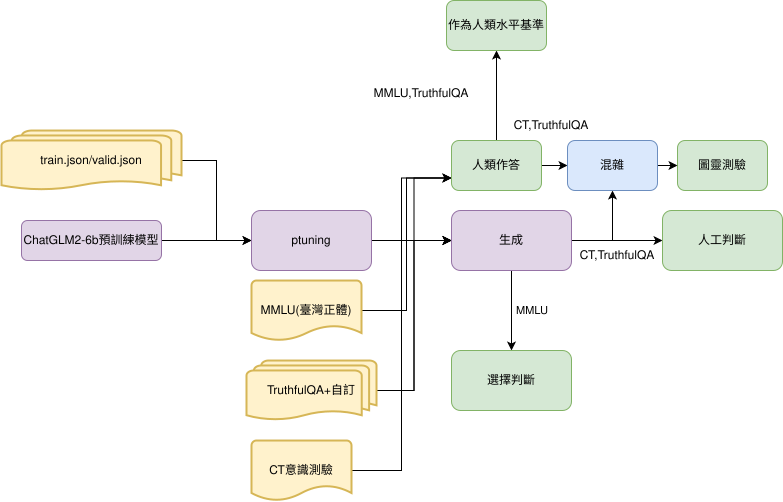
\includegraphics[width=\textwidth]{flowofstudy}%bad resolution
	\subsubsection{資料前處理}
	此部份包含測試資料的取得、題目的翻譯和校正、決定題目的評鑑指標。此部份均由人工處理,本次的資料來源係由研究人員從網路上抓取可信資料並加上情緒特徵,表現出特定角色特色。
	\subsubsection{微調模型訓練}
	資料均正規化之後會被送往模型訓練,本次實驗採用的最多總共有3000步(max\_steps=3000) ,每500次紀錄一次,相關參數紀錄如下:
	\begin{itemize}
		\item gradient\_accumulation\_steps: 16
		\item learning\_rate: 0.01
		\item pre\_seq\_len: 128
	\end{itemize}
	\subsubsection{測驗}
	訓練完成後,模型會依照指示生成出評估內容,之後由人工評斷,結果評估會使用前一小節討論的四種指標評估,各指標因測驗目的不同將會分別陳列。
	\section{肆、研究結果}
	經過訓練後(實際訓練過程如下圖所示\footnote{為確保公平性,此圖中有關使用者資料被抹除}),模型總訓練時間16小時56分鐘,總大小約339MB,訓練次數(epochs)共計685.71次,結束後train loss約為0.336,經過以上測驗結果依測驗種類分類陳列。%maybe change max token:)
	
	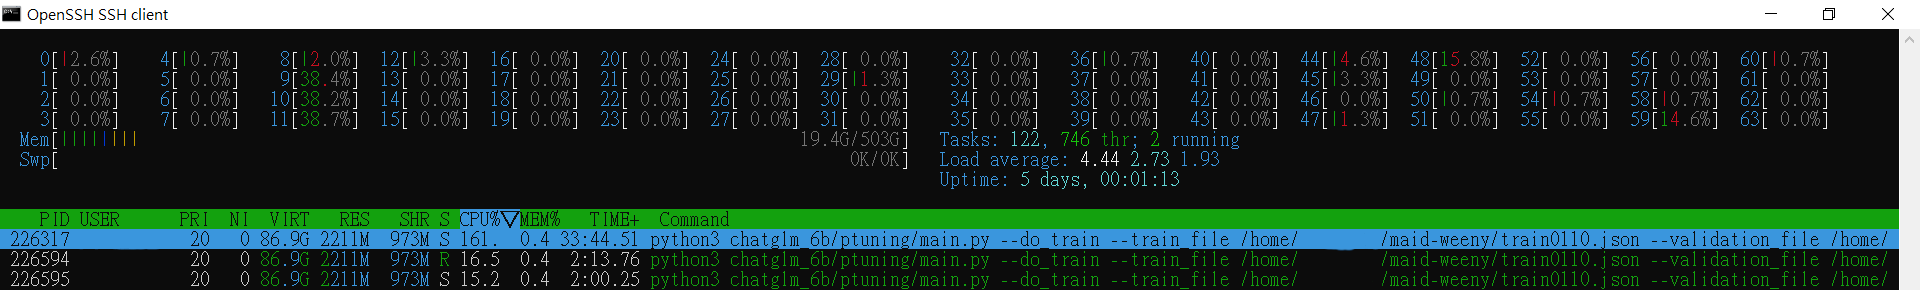
\includegraphics[width=\textwidth]{running}
	%人工討論6*100?
	%標準比對
	\subsection{自我測試比較}
	此處的結果為模型輸出和範例測試資料比較的結果,但需要注意的是,部份範例測試資料旨在評估開放性問答,即可能有多種回答方式的問題,故不應該以此判斷模型成效。
	\begin{table}[H]
		\centering
		\caption{表x、模型自我測試結果}
		\begin{tabular}{lllll}
			& BLEU-4 & ROUGE-1 & ROUGE-2 & ROUGE-L  \\
			500  & 3.5707 & 18.972  & 4.1165  & 14.8251  \\
			1000 & 2.0272 & 18.727  & 3.351   & 11.7919  \\
			1500 & 9.2931 & 25.5811 & 11.3775 & 23.4718  \\
			2000 & 3.2251 & 18.8774 & 2.966   & 14.5734  \\
			2500 & 5.9346 & 23.1986 & 5.332   & 19.5588  \\
			3000 & 4.2043 & 19.2612 & 3.755   & 16.4394 
		\end{tabular}
	\end{table}
	\subsection{TruthfulQA(開放式問答)}
	\subsection{MMLU(封閉性單一選擇問答)}
	\subsection{CT 自我意識測驗}
	\subsection{圖靈測驗}
	此模型在圖靈測驗中表現經整理成混淆矩陣後\footnote{轉換為百分比表示}(下表),其準確率可以高達、F1 score可以高達。
	
	\section{伍、討論}
	\subsection{不同checkpoint比對}
	\subsection{和人類表現比對}
	\subsection{未來展望}
	\begin{quote}
		We can only see a short distance ahead, but we can see plenty there that needs to be done.	--艾倫圖靈
	\end{quote}
	本次研究時間較為緊湊,未能完成不同模型及微調器的比較和對照實驗,實屬可惜,且本次實驗因採用模組為ChatGLM2,於本研究完成時ChatGLM3已經公開釋出。本研究往後將進一步以第三版對照第二版進行研究。
	\section{陸、結論}

	\section{柒、參考文獻資料}
%	\printbibliography
\bibliographystyle{apacite}
\renewcommand{\refname}{}
\bibliography{ref}
\end{CJK*}
\end{document}
